\documentclass[11pt,a4paper]{article}
\usepackage[margin=23mm]{geometry}
\usepackage{amsmath,amssymb,graphicx,booktabs,xcolor,fancyhdr,listings}
\usepackage[hidelinks]{hyperref}
\definecolor{ink}{HTML}{172E48}
\definecolor{teal}{HTML}{176A84}
\definecolor{paperblue}{HTML}{EDF4F7}
\pagestyle{fancy}
\fancyhf{}
\fancyhead[L]{\small\color{teal} STATISTICAL MECHANICS}
\fancyhead[R]{\small\color{ink} BROWNIAN MOTION AND LANGEVIN DYNAMICS}
\fancyfoot[R]{\small\thepage}
\setlength{\headheight}{15pt}
\setlength{\parindent}{0pt}
\setlength{\parskip}{6pt}
\setlength{\abovedisplayskip}{8pt}
\setlength{\belowdisplayskip}{8pt}
\raggedbottom
\lstset{language=Python,basicstyle=\small\ttfamily,backgroundcolor=\color{paperblue},
  columns=fullflexible,keepspaces=true,xleftmargin=8pt,xrightmargin=8pt,
  aboveskip=8pt,belowskip=6pt,showstringspaces=false}
\newcommand{\E}{\mathbb E}
\newcommand{\Var}{\operatorname{Var}}
\newcommand{\dd}{\,\mathrm d}
\newcommand{\N}{\mathcal N}
\newcommand{\figcap}[1]{\par\smallskip{\small\itshape #1}\par}
\begin{document}
{\color{teal}\large Simulation notes}\par
{\color{ink}\Huge\bfseries From Brownian motion\\[3pt] to Langevin dynamics}\par
\vspace{4pt}
{\large A derivation and a guide to the Python simulation}\par
\vspace{8pt}
\noindent\textcolor{teal}{\rule{\linewidth}{1pt}}
\tableofcontents

\section{From a coin flip to a Wiener process}
Take \(n\) independent fair-coin steps per unit time. Each step \(Y_j\) is either
\(+1/\sqrt n\) or \(-1/\sqrt n\). Its mean is zero and its variance is
\(\E[Y_j^2]-(\E[Y_j])^2=1/n\).
Between times \(s\) and \(t\) there are
\(M=\lfloor nt\rfloor-\lfloor ns\rfloor\) steps. Independence makes the
variances add, so the displacement has mean zero and variance \(M/n\to t-s\).
The central limit theorem gives a Gaussian limit for this displacement.
Sums over disjoint time intervals use different flips, so their limiting
increments are independent.

A standard Wiener process \(W_t\) starts at \(W_0=0\), has continuous paths
and independent increments, and satisfies
\[
 W_t-W_s\sim\N(0,t-s),\qquad 0\le s<t.
\]
The coin-flip argument motivates the increment law. The Wiener process also
specifies the continuous-time path, which is almost surely nowhere differentiable.
Here \(\N(\mu,\sigma^2)\) lists the mean and \emph{variance}.

\subsection*{Why a step uses the square root of time}
If \(Z\sim\N(0,1)\), multiplying it by \(c\) multiplies its variance by \(c^2\).
Therefore \(\Delta W=\sqrt{\Delta t}\,Z\) has variance \(\Delta t\).
For example, at \(\Delta t=0.01\) the standard deviation is \(0.1\).
A fresh Gaussian draw per step gives the correct joint distribution at the
sampled times. Lines drawn between those times are a visualization of the grid.
\newpage

\section{Brownian simulation and mean squared displacement}
With \(t_j=j\Delta t\), the Brownian loop adds each Gaussian increment to the
previous position. Store the initial zero so index \(j\) corresponds to time \(t_j\).
\begin{lstlisting}
dt = total_time / total_steps
sd = math.sqrt(dt)
times = [step * dt for step in range(total_steps + 1)]
paths = []
for run in range(num_paths):
    position = 0.0
    path = [position]
    for step in range(total_steps):
        z = random.gauss(0, 1)
        position += sd * z
        path.append(position)
    paths.append(path)
\end{lstlisting}
The mean squared displacement (MSD) uses the same time index from every path.
Since \(W_0=0\) and \(\E[W_t]=0\), the theoretical MSD equals \(\Var(W_t)=t\).
\[
 \widehat{\mathrm{MSD}}(t_j)
 =\frac{1}{N}\sum_{i=1}^N\bigl[W^{(i)}(t_j)-W^{(i)}(0)\bigr]^2
 =\frac{1}{N}\sum_{i=1}^N\mathtt{paths[i][j]}^2.
\]
Pooling every time index would mix distributions with different widths and
include correlated positions from each path. For an endpoint histogram at time
\(t\), take one value per path and compare with \(\N(0,t)\). The 100-path
example below uses \(\Delta t=0.01\) and ends at \(t=1\).

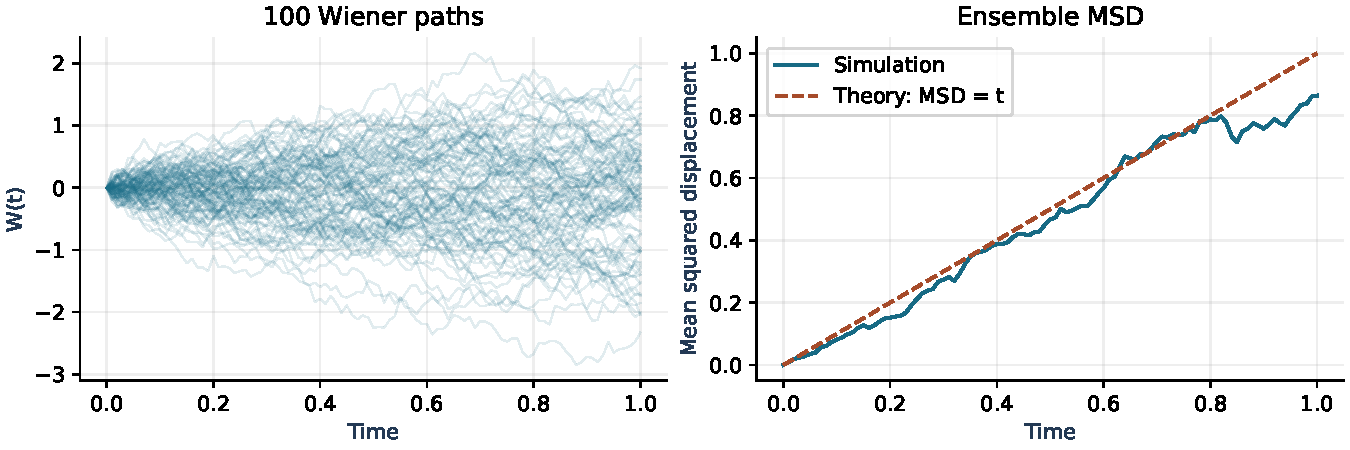
\includegraphics[width=\linewidth]{brownian_example.pdf}
\figcap{Figure 1. Brownian paths and ensemble MSD from a seeded run of the
100-path example. At a fixed time the Monte Carlo standard error of the MSD
is \(t\sqrt{2/N}\), about \(0.141\) at \(t=1\) for this run. This follows from
\(\E[W_t^4]=3t^2\) for a centered Gaussian.}
\newpage

\section{The Langevin equation and thermal noise}
Consider a free particle of mass \(m>0\) in one dimension, coupled to a heat bath
at temperature \(T\). The bath produces viscous drag \(-\gamma V\), with
\(\gamma>0\), and rapidly fluctuating forces. With drag alone, Newton's law gives
\(m\,\mathrm dV/\mathrm dt=-\gamma V\), hence
\(V(t)=V(0)e^{-\gamma t/m}\). Its kinetic energy would decay to zero.
At equilibrium, equipartition assigns one quadratic velocity degree of freedom
mean energy \(k_BT/2\), so
\[
 \frac12m\E[V^2]_{\rm eq}=\frac12 k_BT,
 \qquad \Var(V)_{\rm eq}=\frac{k_BT}{m}
 \quad\text{when }\E[V]_{\rm eq}=0.
\]
The noise represents the net random impulse from the bath. In the white-noise
idealization the impulse over a short interval is proportional to the
Wiener increment. Write
\[
 \mathrm dX_t=V_t\dd t,\qquad
 \mathrm dV_t=-aV_t\dd t+b\dd W_t,\qquad a=\frac{\gamma}{m}.
\]
The velocity is an Ornstein--Uhlenbeck (OU) process. To fix \(b\), apply It\^o's
rule to \(V_t^2\). The quadratic variation of the noise contributes \(b^2\dd t\):
\[
 \mathrm d(V_t^2)=(-2aV_t^2+b^2)\dd t+2bV_t\dd W_t.
\]
The stochastic integral has zero mean. At equilibrium the second moment
satisfies \[0=-2a\E[V^2]_{\rm eq}+b^2.\] Equating it to the equipartition value
sets the fluctuation--dissipation relation
\[
 \frac{b^2}{2a}=\frac{k_BT}{m},
 \qquad
 b=\frac{\sqrt{2\gamma k_BT}}{m}.
\]
Drag removes kinetic energy and thermal noise replenishes it on average.
In the code, \texttt{kBT} is the product \(k_BT\), and \(1/a=m/\gamma\)
sets the relaxation time.

\subsection*{A tool for the variance derivations}
For deterministic \(f(s)\), the integral \(\int_0^t f(s)\dd W_s\) is the
limit of weighted Gaussian increments \(\sum_j f(s_j)\Delta W_j\).
Each sum is Gaussian with mean zero. Independence eliminates cross terms
in its variance, giving \(\sum_j f(s_j)^2\Delta s\). Taking the limit yields
\[
 \Var\!\left(\int_0^t f(s)\dd W_s\right)=\int_0^t f(s)^2\dd s.
\]
This deterministic-integrand case of the It\^o isometry explains both why
the endpoint distributions are Gaussian and why their variances are integrals
of squared weights.
\newpage

\section{Deriving the velocity and position variances}
\subsection*{Velocity from an integrating factor}
Multiply the velocity equation by \(e^{at}\). The product rule cancels the
drag term, giving \(\mathrm d(e^{at}V_t)=be^{at}\dd W_t\).
Integration gives
\[
 V_t=v_0 e^{-at}+b\int_0^t e^{-a(t-s)}\dd W_s.
\]
For fixed \(v_0\), \(\E[V_t]=v_0e^{-at}\). Using the squared-weight rule,
\begin{align*}
 \Var(V_t)
 &= b^2\int_0^t e^{-2a(t-s)}\dd s
  = b^2\int_0^t e^{-2au}\dd u
  = \boxed{\frac{b^2}{2a}(1-e^{-2at})}.
\end{align*}
The factor \(2a\) comes from squaring the exponential weight. With \(v_0=0\),
the width grows from zero and approaches the equipartition variance.

\subsection*{Position from the same Wiener increments}
Integrate the velocity SDE itself. Since \(\int_0^t V_s\dd s=X_t-x_0\),
\[
 V_t-v_0=-a(X_t-x_0)+bW_t.
\]
Substitute the solution for \(V_t\) and write \(W_t=\int_0^t 1\dd W_s\).
Combining the two integrals before taking a variance keeps their shared noise:
\[
 X_t=x_0+\frac{v_0}{a}(1-e^{-at})
     +\frac ba\int_0^t\bigl(1-e^{-a(t-s)}\bigr)\dd W_s.
\]
The first two terms give the mean for fixed \(x_0,v_0\). Squaring the
kernel and integrating each term gives
\begin{align*}
 \Var(X_t)
 &=\left(\frac ba\right)^2\int_0^t(1-e^{-au})^2\dd u\\
 &=\left(\frac ba\right)^2\int_0^t(1-2e^{-au}+e^{-2au})\dd u\\
 &=\boxed{\left(\frac ba\right)^2
 \left[t-\frac{2(1-e^{-at})}{a}+\frac{1-e^{-2at}}{2a}\right]}.
\end{align*}
With \(x_0=v_0=0\), both endpoint means are zero and the position MSD equals
\(\Var(X_t)\). For \(t\ll 1/a\), \(1-e^{-au}\approx au\), so this
from-rest MSD grows as \(b^2t^3/3\). A thermally equilibrated initial velocity
would instead give a leading ballistic term \((k_BT/m)t^2\).
For \(t\gg1/a\) the leading term is \(2Dt\), with
\(D=b^2/(2a^2)=k_BT/\gamma\). For the run at \(t=10\), the full expression
gives \(17.000182\), while the leading term is \(20\).
\newpage

\section{Mapping the Langevin equations to Python}
Euler--Maruyama takes the drift at the beginning of each interval and uses a
Wiener increment with variance \(\Delta t\):
\[
 x_{j+1}=x_j+v_j\Delta t,\qquad
 v_{j+1}=(1-a\Delta t)v_j+b\sqrt{\Delta t}\,Z_j.
\]
The position line comes first so it uses the old \(v_j\). The noise acts
on velocity, and position accumulates those velocities. The code evaluates
\texttt{noise\_scale} once, then draws a new \(Z_j\) for every particle and step.
\begin{lstlisting}
rng = random.Random(42)
noise_scale = b * math.sqrt(dt)

for particle in range(num_particles):
    x = v = 0.0
    positions = [x]
    for step in range(total_steps):
        z = rng.gauss(0, 1)
        x += v * dt
        v += -a * v * dt + noise_scale * z
        if particle < 100:
            positions.append(x)
    if particle < 100:
        pos_stored.append(positions)
    pos_final.append(x)
    velo_final.append(v)
\end{lstlisting}
\texttt{Random(42)} constructs a pseudorandom generator with a fixed seed for
the report run. It is initialized once before the loops, so successive calls
use successive draws. The original \texttt{random.gauss(0, 1)} uses the same
standard normal law through Python's module-level generator. For the current
parameters, \(a=1\), \(b=\sqrt2\), \(\Delta t=10/1000=0.01\), and the
standard deviation of the noise added to velocity in one step is
\(b\sqrt{\Delta t}\approx0.1414\).

\texttt{pos\_stored} holds 100 complete position paths for plotting. In
contrast, \texttt{pos\_final} and \texttt{velo\_final} each hold 10,000 values
sampled at the same final time. The original \texttt{velo\_stored} holds entire
velocity paths, which the endpoint plots never read.

\subsection*{Time-step bias and sampling uncertainty}
Let \(q=1-a\Delta t\). Because each new draw is independent of \(v_j\), the
numerical velocity variance satisfies \(S_{j+1}=q^2 S_j+b^2\Delta t\).
For \(|q|<1\) the stationary value is
\[
 S_\infty=\frac{b^2\Delta t}{1-q^2}
         =\frac{b^2}{2a(1-a\Delta t/2)}.
\]
Here it is about \(1.0050\), compared with the continuous-time limit \(1\).
More particles reduce sampling fluctuations. A smaller step at fixed final
time reduces the discretization bias. For Gaussian endpoints with variance
\(\sigma^2\), the sample mean has standard error \(\sigma/\sqrt N\), and the
variance estimator has standard error approximately \(\sigma^2\sqrt{2/N}\).
\newpage

\section{Example output from the 10,000-particle run}
The following figures use the pasted Langevin update and parameter values,
with the 100-path display, 40-bin histograms, theory overlays, and seed 42.
The horizontal histogram shares the position axis with the trajectory plot.

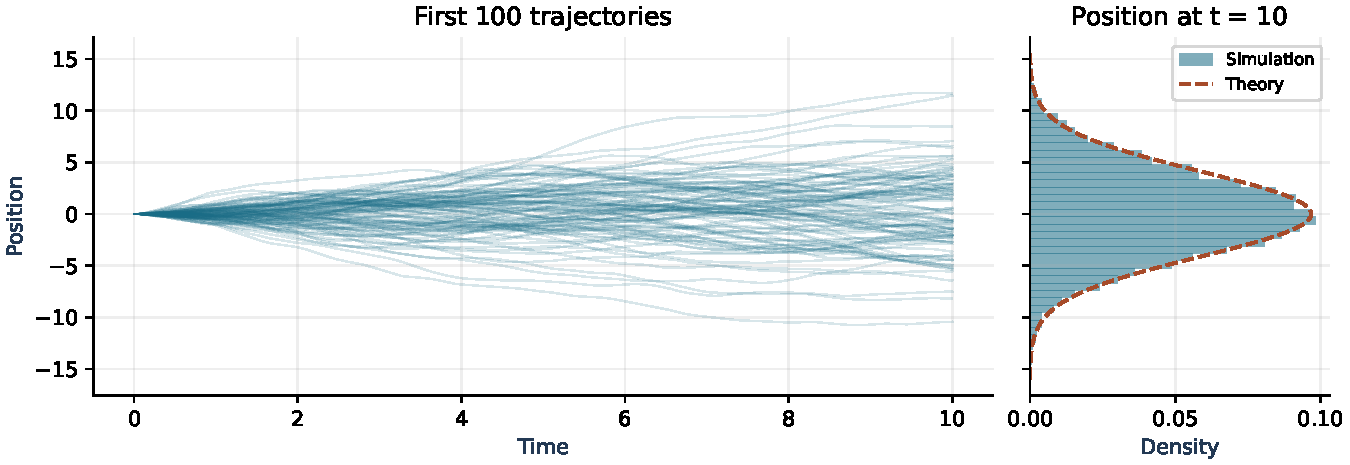
\includegraphics[width=\linewidth]{langevin_position.pdf}
\figcap{Figure 2. The first 100 position trajectories and the final-position
density from all 10,000 particles. The dashed curve uses the full finite-time
position variance.}

\begin{center}
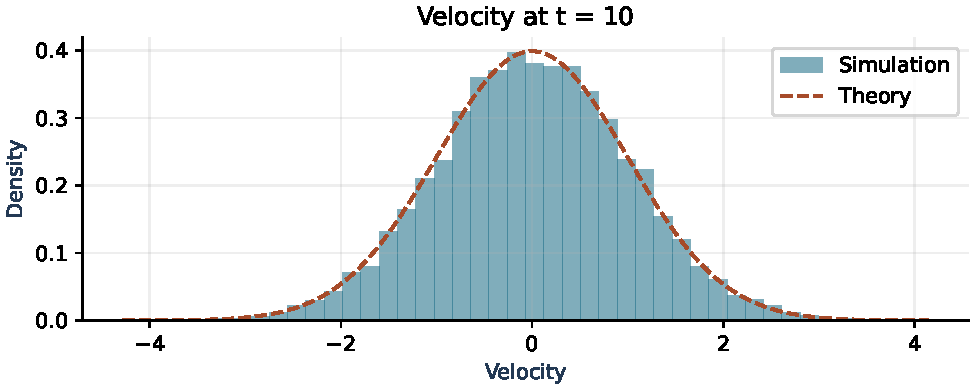
\includegraphics[width=0.69\linewidth]{langevin_velocity.pdf}
\end{center}
\vspace{-7pt}
\figcap{Figure 3. Final velocities from the same particles, with the
continuous-time OU density at \(t=10\).}

\begin{center}
\begin{tabular}{@{}lrrrr@{}}
\toprule
Endpoint & Simulation mean & Theory mean & Simulation variance & Theory variance\\
\midrule
Position & 0.025002 & 0 & 17.212328 & 17.000182\\
Velocity & 0.012620 & 0 & 1.006243 & 1.000000\\
\bottomrule
\end{tabular}
\end{center}
\figcap{Table 1. Endpoint statistics from the run shown above. The theory
column uses continuous time with \(x_0=v_0=0\).}
\newpage

\section{How the code builds the theory overlays}
A centered Gaussian with variance \(s^2\) has probability density
\[
 p(y)=\frac{1}{\sqrt{2\pi s^2}}\exp\!\left(-\frac{y^2}{2s^2}\right).
\]
\texttt{NormalDist} expects the standard deviation \(s\). Pass the square
root of each theoretical variance, then evaluate \texttt{pdf} at closely spaced
values along the variable's axis.
\begin{lstlisting}
t = times[-1]
var_v = b**2 / (2*a) * (1 - math.exp(-2*a*t))
var_x = (b/a)**2 * (
    t - 2*(1 - math.exp(-a*t))/a
    + (1 - math.exp(-2*a*t))/(2*a)
)
theory_x = statistics.NormalDist(0, math.sqrt(var_x))
theory_v = statistics.NormalDist(0, math.sqrt(var_v))
\end{lstlisting}
With \texttt{density=True}, a bin containing \(c\) values and having width
\(h\) is drawn with density \(c/(Nh)\). The total area of the bars is one,
matching the scale of the PDF. In the horizontal histogram, the variable is
on the vertical axis, so the plotted coordinates are \((p(x),x)\).
\begin{lstlisting}
ax_hist.hist(pos_final, bins=40, density=True,
             orientation="horizontal", alpha=0.5)
low, high = ax_hist.get_ylim()
xs = [low + (high - low) * i / 299 for i in range(300)]
ax_hist.plot([theory_x.pdf(x) for x in xs], xs, "--")
\end{lstlisting}
For the velocity histogram, \texttt{get\_xlim()} supplies the velocity range
and the curve uses the usual coordinate order \((v,p(v))\).
\texttt{sharey=True} aligns position values across both panels.

The printed statistics use \texttt{statistics.mean} and
\texttt{statistics.pvariance}. For endpoint values \(y_i\) these compute
\[
 \bar y=\frac{1}{N}\sum_i y_i,\qquad
 \widehat{\Var}(y)=\frac{1}{N}\sum_i(y_i-\bar y)^2.
\]
The MSD about zero satisfies \(N^{-1}\sum_i y_i^2=\widehat{\Var}(y)+\bar y^2\).
The theoretical means are exactly zero here, while a finite simulation
usually has a small nonzero sample mean.

\subsection*{Reproducing the figures}
The source archive includes \texttt{make\_figures.py} and the generated vector
figures. Run \texttt{python make\_figures.py} with Matplotlib installed to
regenerate the plots and print the endpoint statistics. Compile
\texttt{brownian\_langevin.tex} twice with LaTeX to populate the contents.
\end{document}
